\chapter{The HELIOS Concept}
\label{HELIOS_Concept}
%The HELIOS spectrometer is specifically designed to address the challenges encountered in inverse kinematics. 
The HELIcal Orbit Spectrometer (HELIOS) offers a new way of studying reactions in inverse kinematics that has several advantages over the detection methods mentioned in Chapt.~\ref{standards}.  The conceptual principle of HELIOS is introduced in Refs.~\cite{Schiffer_1998,Schiffer_2003}; the proposed design and performance characteristics are laid out in Refs.~\cite{Wuosmaa_2003,Wuosmaa_2007}, and the technical realization and the details of the experimental commissioning are presented in Ref.~\cite{Lighthall_2010}.  The goal of this chapter is to summarize, derive, and expand on the key mathematical concepts presented in these references.
\begin{figure}[!ht]
\centering
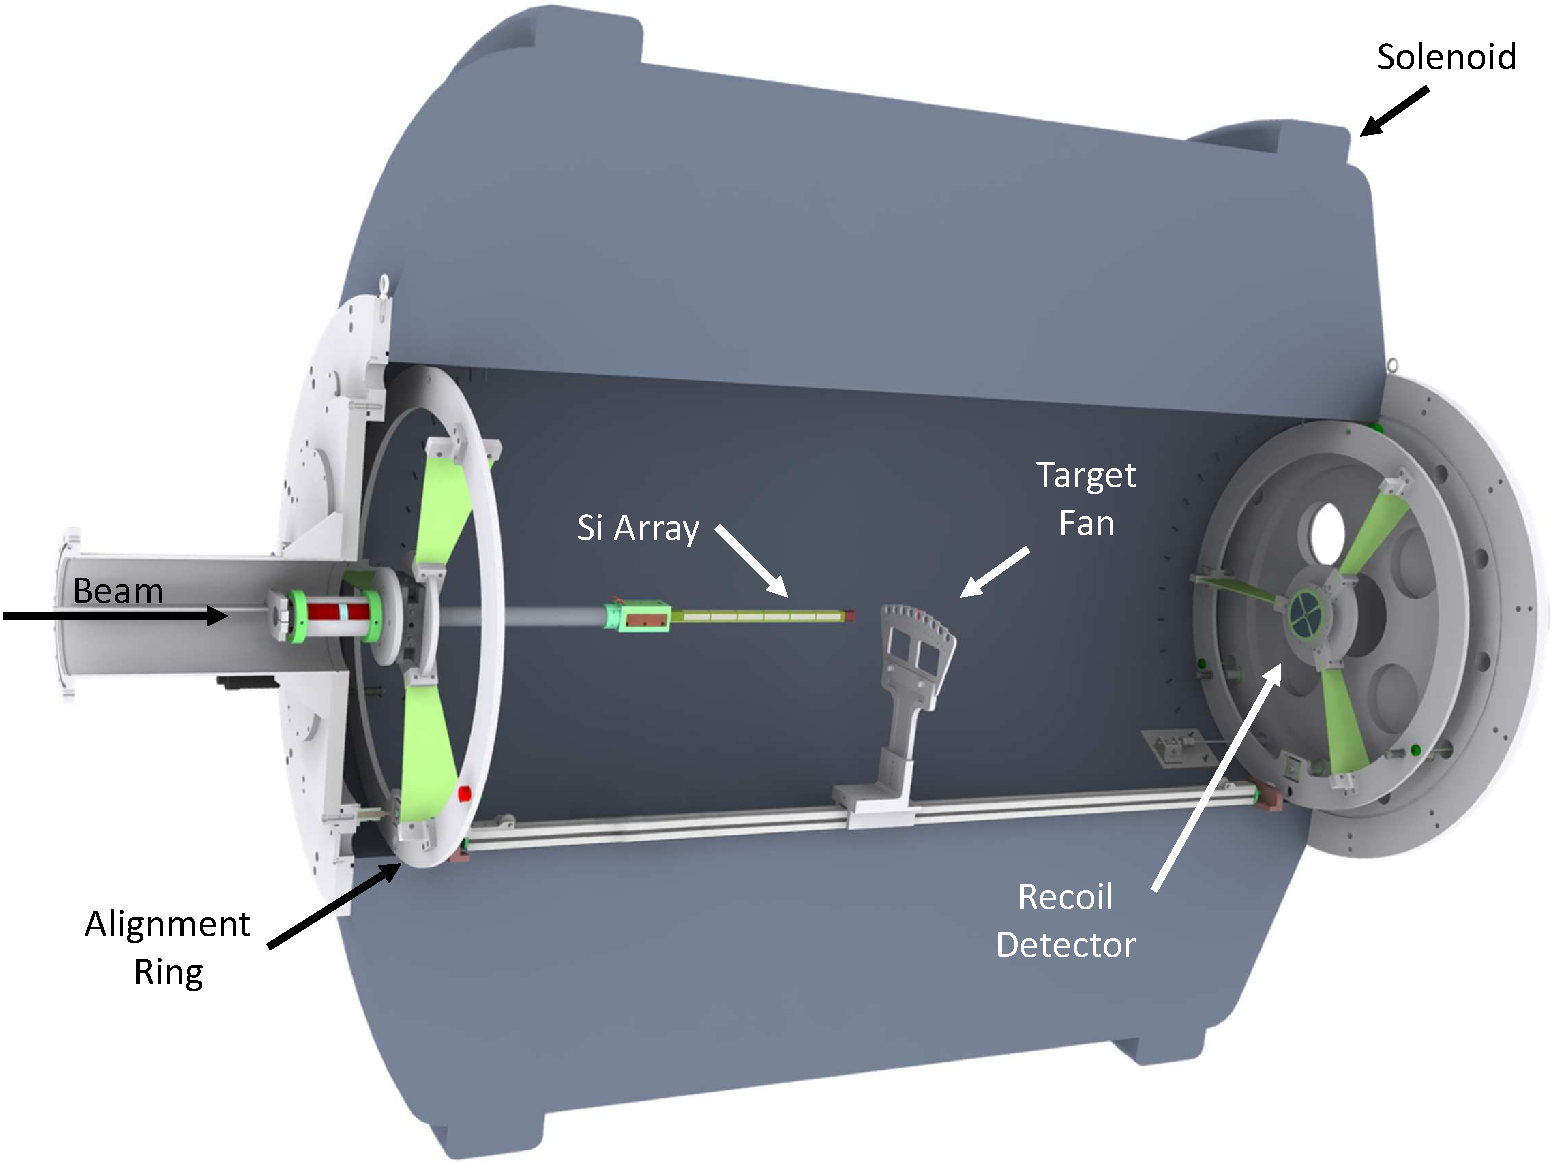
\includegraphics[width=\linewidth,height=0.5\textheight,keepaspectratio]{../NIM_Paper/Figures/18pt_rot3}
\caption[Cutaway schematic view of HELIOS in the ``($d$,$p$)'' configuration]{Cutaway schematic view of HELIOS in the ``($d$,$p$)'' configuration.  The accelerated beam enters from left.  Shown are the light-ion silicon detector array suspended on the upstream alignment ring, rotating target fan, and heavy-recoil detector.  Mechanical design by S.~Heimsath.  3D rendering by B.~J.\ DiGiovine.  This figure also appears in Ref.~\cite{Lighthall_2010}.}
\label{schematic}
\end{figure}

Schematically, HELIOS is based on a large-bore superconducting solenoid, as shown in an engineering model in Fig.~\ref{schematic}.  Accelerated heavy-ion beams enter the solenoid along the magnetic axis, passing through a hollow detector array.  The beam then intercepts a ``light-ion'' target, also on the magnetic axis.  In the configuration shown in the figure, charged reaction products ejected rearward in the laboratory frame---that is, $\theta_\mathrm{lab}>90^\circ$---move in helical orbits to the detector array.  Beam-like recoils are kinematically focused forward in a narrow cone and intercepted by a detector array for identifying heavy ions.
\section{Solenoid Kinematics}
\label{solkin}
The solenoid used in HELIOS produces what is effectively an uniform axial magnetic field.  The technical specifications of the solenoid as well as the features of the magnetic field are discussed in detail in Chapt.~\ref{sol}.  When a reaction occurs within such a magnetic field, the trajectories of the reaction products are simplified due to the constraints of cyclotron motion.  With the solenoid axis aligned collinearly with the beam axis, ions emitted at the target travel in helical orbits under the influence of the magnetic field and return to the magnetic field axis.
\subsection{Coordinates}
\label{coord}
The particle trajectories are defined by the orientation of the laboratory velocity $\vec{v}_\mathrm{lab}$ relative to the solenoid axis.  The symmetry of the solenoid defines a cylindrical coordinate system ($z$,$\rho$,$\phi$), with the beam traveling in the $+z$ direction and the azimuthal angle $\phi=0$ defined relative to ``beam right'' (the $+x$ axis).  Furthermore, the coordinate convention used with HELIOS defines the $+y$ axis as ``up'' yielding a left-handed coordinate system.  With this convention in mind, the laboratory velocity may be written as 
\begin{equation}
\vec{v}_\mathrm{lab}=v_\parallel \hat{z}+v_\perp \hat{\rho}
\label{lab_vel}
\end{equation}
with $v_\parallel$ and $v_\perp$ defined in terms of the polar angle as
\begin{equation}
\begin{split}
v_\perp&\equiv v_\mathrm{lab}\sin(\theta_\mathrm{lab})\\
&=v_0\sin(\theta_\mathrm{cm})\\
\end{split}
\end{equation}
and
\begin{equation}
\begin{split}
v_\parallel &\equiv v_\mathrm{lab}\cos(\theta_\mathrm{lab})\\
&=V_\mathrm{cm}+v_0\cos(\theta_\mathrm{cm})\\
\end{split}
\label{eq:vpara}
\end{equation}
 as illustrated in Fig.~\ref{vector}.  In these equations $v_0$ retains its definition from Eq.~\ref{kin_v0}.
\begin{figure}
\begin{center}
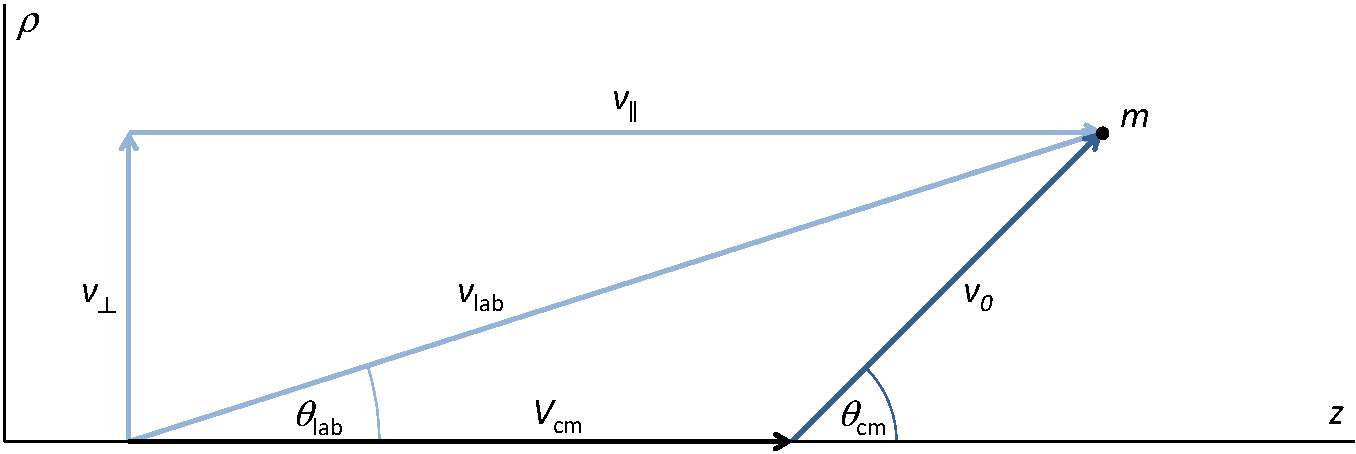
\includegraphics[width=\columnwidth]{kin_fig_4c}
\setlength{\unitlength}{0.125\columnwidth}
%\fbox{
%\begin{picture}(4.5,2.75)(.25,.125)
%\thinlines
%\put(0.5,0.50){\line(1,0){3.75}}%z
%\put(0.5,0.50){\line(0,1){2}}   %rho
%\thicklines
%\put(1,0.5){\vector(1,0){2}}    %Vcm
%\put(1,0.5){\vector(3,2){3}}    %vlab
%\put(3,0.5){\vector(1,2){1}}    %v0

%\put(2,0.3){$V_\mathrm{cm}$}
%\put(2,1.5){$v_\mathrm{lab}$}
%\put(3.65,1.5){$v_0$}
%\put(1.4,0.6){$\theta_\mathrm{lab}$}
%\put(3.2,0.6){$\theta_\mathrm{cm}$}
%\put(4.4,0.45){$z$}
%\put(.45,2.7){$\rho$}
%\end{picture}
%}%end fbox
\end{center}
\caption[Vector diagram of relevant velocities of the mass $m$ ejectile]{Vector diagram of relevant velocities of the mass $m$ ejectile. $\vec{v_\mathrm{lab}}=\vec{V_\mathrm{cm}}+\vec{v_0}$ with $v_\mathrm{lab}$ the ejectile velocity in the laboratory, $V_\mathrm{cm}$ the velocity of the center-of-mass, and $v_0$ the ejectile velocity in the center-of-mass.  The velocity projections $v_\perp$ and $v_\parallel$ are defined as illustrated.}%
\label{vector}%
\end{figure}
\subsection{Cyclotron Motion}
The velocity component perpendicular to the solenoid axis $v_\perp$ defines the radius of cyclotron motion 
\begin{equation}
\begin{split}
r=v_{\perp}\frac{m}{\mathscr{B}q}\\
\end{split}
\label{cyc_rad}
\end{equation}
for a particle of mass $m$ and charge $q$ traveling in a field of strength $\mathscr{B}$.  A related quantity, the cyclotron period $T_\mathrm{cyc}$, is fixed by the mass-to-charge ratio of the particle and the magnetic field strength. 
\begin{equation}
\begin{split}
T_\mathrm{cyc}&=\frac{2\pi r}{v_{\perp}}\\
       &=\frac{2\pi}{\mathscr{B}} \left(\frac{m}{q}\right)
\end{split}
\label{Tcyc}
\end{equation}
\par The position at which particles return to the solenoid axis varies according to their velocity parallel to the magnetic field $v_\parallel$.  As such, HELIOS disperses ions by $v_\parallel$.  For a given value of $(m/q)$ and magnetic field, the axial path length (return distance) is given by
\begin{equation}
\begin{split}
z_n&=v_\parallel (n \times  T_\mathrm{cyc})
\end{split}
\label{loops}
\end{equation}
after executing $n$ number of orbits.  For purposes of nomenclatural clarity, it is useful at this point to introduce the variable $z_1$, the point at which a particle undergoing a single orbit intercepts the solenoid axis.

\section{Determining the Center-of-mass Quantities}
Particles are detected within HELIOS along the length of a hollow array of position sensitive silicon detectors (PSDs) suspended on the solenoid axis.  This detector arrangement represents a fundamental departure from the tradition measurement approach wherein the scattering angle $\theta_\mathrm{lab}$ is measured.  When a light ion intercepts an active portion of the silicon detector array, three quantities are measured: the energy $E$, the time of flight $t$, and the axial position $z$.    From these measured quantities, the 
center-of-mass quantities of energy $E_\mathrm{cm}$ and emission angle $\theta_\mathrm{cm}$ are derived.  
\subsection{Excitation Energy}
The transformation of the energy of the ejectile in the laboratory frame to the energy in the center-of-mass frame can be reduced to a linear transformation.  Substituting Eq.~\ref{eq:vpara} into Eq.~\ref{elab}, the laboratory energy $E_\mathrm{lab}$ can be rewritten as
%Starting with %the non-relativistic definition of kinetic energy, $E_\mathrm{lab}=\frac{1}{2} m(v_\mathrm{lab})^2$, %the equations of \S\,\ref{coord} can be used to rewrite 

\begin{equation}
\begin{split}
%E_\mathrm{lab}&=%\frac{1}{2} m(v_\parallel^2+v_\perp^2 )\\
%&=\frac{1}{2} m\left[(V_\mathrm{cm} +v_0 \cos(\theta_\mathrm{cm}))^2+v_0^2 \sin^2(\theta_\mathrm{cm})\right]\\
%&=\frac{1}{2} m\left[V_\mathrm{cm}^2 +2V_\mathrm{cm}v_0 \cos(\theta_\mathrm{cm})+v_0^2\cos^2(\theta_\mathrm{cm})+v_0^2 \sin^2(\theta_\mathrm{cm})\right]\\
%\frac{1}{2} m\left[v_0^2+V_\mathrm{cm}^2 +2V_\mathrm{cm}v_0 \cos(\theta_\mathrm{cm})+\right]\\
E_\mathrm{lab}&=\frac{1}{2} m\left[v_0^2+V_\mathrm{cm}^2 +2V_\mathrm{cm}v_0 \cos(\theta_\mathrm{cm})\right]\\
&=\frac{1}{2} m\left\{v_0^2+2V_\mathrm{cm}[v_0 \cos(\theta_\mathrm{cm})+V_\mathrm{cm}-V_\mathrm{cm}]+V_\mathrm{cm}^2 \right\}\\
%&=\frac{1}{2} m\left[V_\mathrm{cm}^2 +2V_\mathrm{cm}v_\parallel-2V_\mathrm{cm}^2+v_0^2\right]\\
&=\frac{1}{2} m\left(v_0^2+2V_\mathrm{cm}v_\parallel -V_\mathrm{cm}^2\right).
\end{split}
\label{elab_of_vpara}
\end{equation}

A given beam energy fixes the value of $V_\mathrm{cm}$ and, given a reaction and transition, $v_{0}$ is fixed.  Therefore, the measured energy $E_\mathrm{lab}$ depends linearly according to $v_\parallel$, the laboratory velocity parallel to the beam axis.  Assuming the particles are detected on the magnetic axis, this quantity has a value of $v_\parallel=z_n/(n T_\mathrm{cyc})$.  Inserting this expression into Eq.~\ref{elab} and   rearranging to solve for the center-of-mass energy, defined as $E_\mathrm{cm}=\frac{1}{2}m( v_0)^2$, gives the center-of-mass energy as a linear offset from the laboratory energy. 
\begin{equation}
E_\mathrm{cm}=E_\mathrm{lab}+\frac{1}{2} mV_\mathrm{cm}^2-\frac{m V_\mathrm{cm}}{n T_\mathrm{cyc}}z_n
\label{ecm}
\end{equation}
%Measuring the position of axis intercept relative to the target, combined with the fixed time-of-flight, disperses particles , their   The position of axis intercept $z$, together with the measured laboratory energy, defines the center-of-mass angle and energy of the reaction in a linear relationship
The excitation energy $E_x$ is then derived from the center-of-mass energy by correcting for the recoil mass of the residual nucleus. Substituting Eq.~\ref{eq:ecm} into Eq.~\ref{eq:ecmtotal} and solving for $E_x$ yields
\begin{equation}
E_x=T_\mathrm{cm}+Q-E_\mathrm{cm}\frac{m+M}{M}
\label{eq:recoil_mass}
\end{equation}

\subsection{Emission Angle}
In order to study the angular distributions for transitions to different excited states, it is necessary to calculate the scattering angle in the center-of-mass $\theta_\mathrm{cm}$.  With reference to Fig.~\ref{vector}, the center-of-mass angle is readily obtained using the law of cosines.
%Equation moved to kinematics chapter.

Starting with the %velocity relation given by the low of cosines in 
Eq.~\ref{eq:law_of_cosines} and solving for $\theta_\mathrm{cm}$ yields
\begin{equation}
\begin{split}
\theta_\mathrm{cm}=&\arccos\left(\frac{v_\mathrm{lab}^2-v_0^2-V_\mathrm{cm}^2}{2v_0 V_\mathrm{cm}}\right).
%\theta_\mathrm{cm}=&\arccos\left[\frac{\frac{2}{m}(E_\mathrm{lab}-E_\mathrm{cm})-V_\mathrm{cm}^2}{\sqrt{2 E_\mathrm{cm}/m}V_\mathrm{cm}}\right]
\end{split}
\label{costhetacm}
\end{equation}
This is the familiar result of two-body kinematics from classical mechanics (\textit{cf}.~\citet[Eq.~3.109]{Goldstein_2002}).
As alluded to earlier, $V_\mathrm{cm}$ is fixed by the bombarding energy of the beam.  Once the excitation energy is determined using Eq.\,\ref{ecm}, the value of $v_0$ is fixed.  Thus, for a given transition, the center-of-mass angle is uniquely determined by $v_\mathrm{lab}$, which is calculated from the measured laboratory energy $E_\mathrm{lab}$.  

\section{Advantages}
The principles laid out in this chapter describing the HELIOS concept provide a number of advantages over traditional detection techniques.
\subsection{Particle Identification}
\par The cyclotron period is an especially important quantity because it defines the time of flight for the detected particles and provides particle identification.  The time-of-flight is approximately%ed by 
\begin{equation}
T_\mathrm{cyc}=65.1\,\textrm{ns}\times \frac{An}{q\mathscr{B}}
\end{equation}
with $A$ the atomic mass number, $n$ is the number of orbits, $q$ in units of $e$, and $\mathscr{B}$ in Tesla.  Table~\ref{flight_times} gives the cyclotron periods ($n=1$) for the H and He isotopes with $A\leq 4$ for %$\mathscr{B}=2.0$\,T.
a variety of field strengths.  The minimum separation in ns of the cyclotron periods for these light ions is approximately  $32.6/\mathscr{B}$, where $\mathscr{B}$ is in units of T.  With a field strength of $\mathscr{B}=2.0$\,T, this separation is 16.3\,ns; timing resolution of this magnitude is readily achievable with typical silicon detectors.  Thus, by means of measuring the time of flight, HELIOS solves the problem of particle identification of light-ion reaction products at low energy.  The particle identification is valid up to ambiguities of $An/q$.
\begin{table}
  \begin{center}
    \begin{tabular}{cccc}
      \hline
      \multicolumn{1}{c}{\multirow{2}{*}{Ion}}  &
    	\multicolumn{3}{c}{$T_\mathrm{cyc}$ (ns)}\\ \cline{2-4}
    	%&$q\mathscr{B}/n=1$\,e$\cdot$T&2\,e$\cdot$T&3\,e$\cdot$T\\\hline \hline 
    	&$\mathscr{B}/n=1$\,T&2\,T&3\,T\\\hline \hline 
      $p$&65.6&32.8&21.9\\
      $^3$He&98.2&49.1&32.7\\
      $\alpha$&130.3&65.2&43.4\\
      $d$&131.2&65.6&43.7\\
      $t$&196.4&98.2&65.5\\\hline
    \end{tabular}
    \label{flight_times}
    \caption[Cyclotron periods $T_\mathrm{cyc}$ for typical reaction products for a variety of field strengths]{Cyclotron periods $T_\mathrm{cyc}$ for typical reaction products for a variety of field strengths.}
  \end{center}
\end{table}
\subsection{\texorpdfstring{$Q$-value Resolution}{Q-value Resolution}}
The most significant feature of the HELIOS concept is that it avoids the problem of kinematic compression introduced in \S\,\ref{kin_comp}.  Instead of detecting ions %over a range of 
at fixed laboratory angles, the ions transported by the magnetic field within HELIOS are %measured over a range of 
detected at 
fixed axial positions.  Eq.~\ref{ecm} gives a linear relationship between the measured quantities $E_\mathrm{lab}$ and $z$ and the derived quantity $E_\mathrm{cm}$.  This linear relationship between the laboratory quantities and the center-of-mass system is the key to the enhanced $Q$-value resolution of HELIOS.  Table~\ref{helios_error} shows the calculated $Q$-value resolution for a number of reactions based on the HELIOS concept.  Following the discussion in \S\,\ref{res_prop}, the contributions are calculated assuming energy measurement uncertainties of $\delta E_\mathrm{lab}=40$\,keV~FWHM, and an uncertainty in the beam energy of 0.14\%. In addition, the contribution from the uncertainty of the position is based on $\delta z=1.0$\,mm~FWHM.  As can be seen in the table, the dominant contribution to the $Q$-value resolution is the intrinsic detector resolution, as was the case in normal kinematics.

\begin{table*}%
  \centering
  \begin{tabular}{,......rr}		
    \hline
    \multicolumn{1}{c}{\multirow{2}{*}{Reaction}}  &
    \multicolumn{1}{c}{$E_1/A_1$}  &
    \multicolumn{1}{c}{$\mathscr{B}$}  &
    \multicolumn{1}{c}{$\theta_\textrm{lab}$} & 
    \multicolumn{3}{c}{Origin of contribution}  &
    \multicolumn{2}{c}{$\delta E_\textrm{cm}$}  \\  \cline{5-7}
    &\multicolumn{1}{c}{(\AMeV)}&
    \multicolumn{1}{c}{(T)}&
    \multicolumn{1}{c}{(deg)} & 
    \multicolumn{1}{c}{$\delta z$}  &  
    \multicolumn{1}{c}{$\delta E_\textrm{lab}$} & 
    \multicolumn{1}{c}{$\delta E_1$} & 
    \multicolumn{1}{c}{$\Sigma_\mathrm{quad}$} &
    \multicolumn{1}{c}{$\Sigma_\mathrm{covar}$} \\
    \hline \hline 
    d(^{28}\textrm{Si},p)^{29}\textrm{Si} 	& 6.02 & 2.00 & 157.9 &11 & 40 & 13 & 43 & 32\\
    d(^{12}\textrm{B},p)^{13}\textrm{B} 	 &6.24 & 1.04 & 155.2 &5 & 40 & 11 & 42 & 37\\
    d(^{132}\textrm{Sn},p)^{133}\textrm{Sn}	 &4.78 & 2.00 & 149.0 &10 & 40 & 10 & 42 & 31\\
    d(^{124}\textrm{Sn},^3\textrm{He})^{123}\textrm{In} 	 &13.00 & 2.73 & 21.5 &45 & 40 & 38 & 71 & 38\\
    p(^{77}\textrm{Kr},d)^{76}\textrm{Kr}  	 &30.00 & 2.00 & 15.1 &24 & 40 & 51 & 70 & 54\\
    \hline
  \end{tabular}
  \caption[Calculated contributions to the uncertainty of $E_\textrm{cm}$ for measurements using HELIOS]{Calculated contributions to the uncertainty of $E_\textrm{cm}$ for measurements using HELIOS.  For experiments that have already been preformed, the actual magnetic field value is used; for experiments that have not been run---$^{132}$Sn and $^{77}$Kr---a 2.00\,T field is assumed.  Values are calculated in keV~FWHM for $\theta_\mathrm{cm} = 10^\circ$.  The quadratic sum $\Sigma_\mathrm{quad}$ and the sum including the covariant term $\Sigma_\mathrm{covar}$ are given.}
  \label{helios_error}
\end{table*}

\subsubsection{Energy Separation}
\label{energysep}
At a fixed $z$ position, kinematic loci are separated %, by definition,
 by their laboratory energy $\Delta E_\mathrm{lab}=(E_\mathrm{lab}-E_\mathrm{lab}^\prime)$.  This quantity is related to the center-of-mass energy separation by
\begin{equation}
\begin{split}
\Delta E_\mathrm{lab}%&=\left[E_\mathrm{cm}-\frac{1}{2} mV_\mathrm{cm}^2+\frac{m V_\mathrm{cm}}{T_\mathrm{cyc}}z_1\right]_1-\left[E_\mathrm{cm}-\frac{1}{2} mV_\mathrm{cm}^2+\frac{m V_\mathrm{cm}}{T_\mathrm{cyc}}z_1\right]_2\\
&=\left[E_\mathrm{cm}-\frac{1}{2} mV_\mathrm{cm}^2+\frac{m V_\mathrm{cm}}{T_\mathrm{cyc}}z_1\right]-\left[E_\mathrm{cm}^\prime-\frac{1}{2} mV_\mathrm{cm}^2+\frac{m V_\mathrm{cm}}{T_\mathrm{cyc}}z_1^\prime\right]%\\
%&=\Delta E_\mathrm{cm}
\end{split}
\label{eq:delta_e}
\end{equation}
in which the second term in the bracketed expressions is constant for a given bombarding energy and the last term is constant for fixed $z$.  Taking the difference, these terms drop out and we are left with
\begin{equation}
\Delta E_\mathrm{lab}=\Delta E_\mathrm{cm}.
\label{eq:no_comp}
\end{equation}
Comparing this expression to Eq.~\ref{eq:compress}, on sees the ``compression'' coefficient leading the $\Delta E_\mathrm{cm}$ term is identically equal to $1$ and is independent of scattering angle.  Hence, the separation between kinematic groups corresponding to different energy levels in the residual nucleus at a fixed $z$ is the same as the energy spacing in the center-of-mass frame.  Put another way, with measurements made with HELIOS, there is no kinematic compression. 
This result arises from the constant slope of the kinematic loci, given by
\begin{equation}
\begin{split}
\frac{\partial E_\mathrm{lab}}{\partial z}&=\frac{m V_\mathrm{cm}}{nT_\mathrm{cyc}}
\end{split}
\label{slopeEcm}
\end{equation}
which is independent of $z$ and the reaction $Q$-value and hence is free from kinematic compression. Substituting Eqs.~\ref{Vcm} and \ref{Tcyc} into this expression one also sees the slope is independent of the ejectile mass $m$.
\begin{equation}
\begin{split}
\frac{\partial E_\mathrm{lab}}{\partial z}&=\frac{q\mathscr{B}}{2\pi n}\sqrt{\frac{2 E_1}{m_1}}\left(\frac{m_1}{m_1+m_2}\right)\\
&\approx 2.21\,\textrm{keV/mm} \times \frac{q \mathscr{B}}{n}\sqrt{\frac{E_1}{A_1}}\left(\frac{A_1}{A_1+A_2}\right)
\end{split}
\label{slope_calc}
\end{equation}
where $A_1$ and $A_2$ are the atomic mass numbers of the beam and the target nuclei, respectively; $q$ in units of $e$, and $\mathscr{B}$ in Tesla.  In the limit of inverse kinematics $m_1\gg m_2$, the term in the parentheses is equal to one.  Table~\ref{slopes} gives slopes for the H and He isotopes for a number of field strengths and bombarding energies.

\begin{table}
  \begin{center}
    \begin{tabular}{........}
      \hline
      \multicolumn{1}{c}{$E_1/A_1$(\AMeV)}%&$\mathscr{B}=1$\,T&2\,T&3\,T\\\hline \hline %\\[-2ex]
      &\multicolumn{7}{c}{$q\mathscr{B}/n$ (e$\cdot$T)}\\ \cline{2-8}
      &\multicolumn{1}{c}{0.5}
      &\multicolumn{1}{c}{1.0}
      &\multicolumn{1}{c}{1.5}
      &\multicolumn{1}{c}{2.0}
      &\multicolumn{1}{c}{3.0}
      &\multicolumn{1}{c}{4.0}
      &\multicolumn{1}{c}{6.0}\\\hline \hline 
%      5&4.9& 9.8&14.7\\
%      10&6.9&13.9&20.8\\
%      15&8.5&17.0&25.5\\
%      20&9.8&19.6&29.4\\
			5  & 2.4 & 4.9 &  7.3 &  9.8 & 14.7 & 19.6 & 29.4 \\
			10 & 3.5 & 6.9 & 10.4 & 13.8 & 20.8 & 27.7 & 41.5 \\
			15 & 4.2 & 8.5 & 12.7 & 17.0 & 25.4 & 33.9 & 50.9 \\
			20 & 4.9 & 9.8 & 14.7 & 19.6 & 29.4 & 39.2 & 58.7 \\ \hline
    \end{tabular}
    \label{slopes}
    \caption[Typical slopes of $E_\mathrm{lab}$ vs. $z$ with HELIOS]{Typical slopes of $E_\mathrm{lab}$ vs. $z$ with HELIOS.  Values are given in keV/mm for various bombarding energies and parameter values $q=1$, 2\,e; $\mathscr{B}=1$, 2, 3\,T; and $n=1$,2.}
  \end{center}
\end{table}

The effect of kinematic compression as exhibited by 
%This effect in 
HELIOS
%, or rather, the lack thereof 
is illustrated in Fig.~\ref{helios_basic}.   In practice, this effect is utilized by correcting for the slope of the kinematic curves by means of Eq.~\ref{ecm} and projecting onto the energy axis% to determine the center-of-mass energy
.  The intercept of these lines corresponds to the energy at $z=0$, or equivalently $\theta_\mathrm{lab}=90^\circ$, and is given by
%\begin{equation}
%\begin{split}
%v_\parallel&=0\\
%&=V_\mathrm{cm}+v_0\cos(\theta_\mathrm{cm})\\
%\cos(\theta_\mathrm{cm})&=\frac{-V_\mathrm{cm}}{v_0}\\
%\end{split}
%\label{theta90}
%\end{equation}
%Therefore, the intercept $b$ is given by
\begin{equation}
\begin{split}
%v^2&=(v_\parallel^2+v_\perp^2)\\
%&=v_\perp^2\\
%&=[v_0\sin(\theta_\mathrm{cm})]^2\\
%&=v_0^2\sin^2\left[\arccos\left(\frac{-V_\mathrm{cm}}{v_0}\right)\right]\\
%&=v_0^2\left[1-\left(\frac{-V_\mathrm{cm}}{v_0}\right)^2\right]\\
%&=v_0^2-V_\mathrm{cm}^2\\
%b
E_\mathrm{lab}\big|_{z=0}&=E_\mathrm{cm}-\frac{1}{2}m V_\mathrm{cm}^2.
\end{split}
\label{y_intercept}
\end{equation}
This value is independent of the number of orbits and the resultant spectrum is then independent of $z$. 

\begin{figure}[t]%
\centering
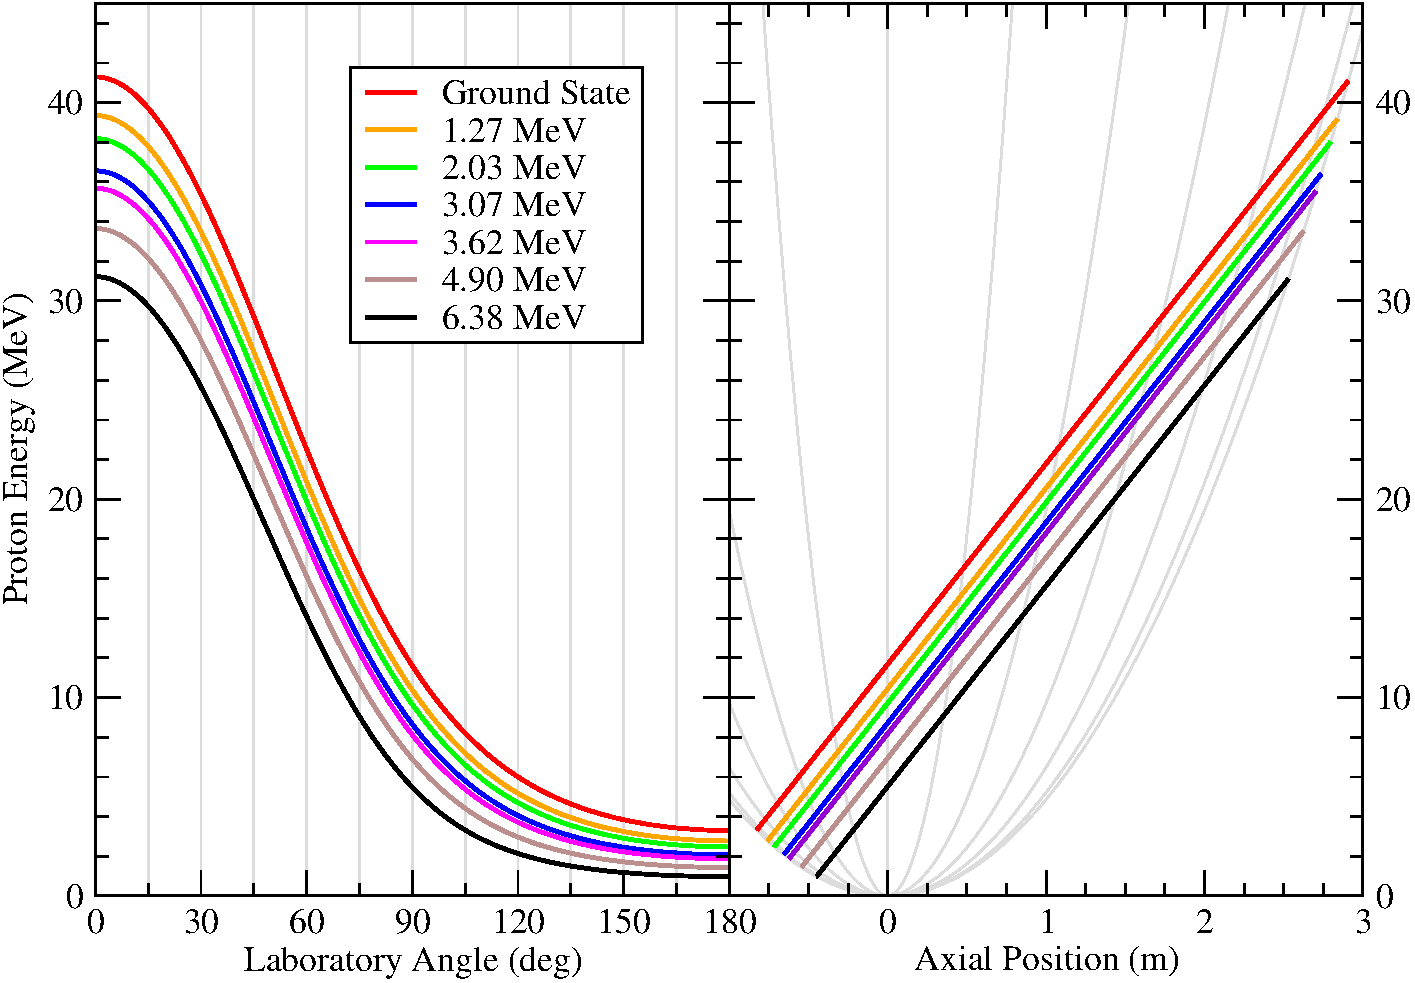
\includegraphics[keepaspectratio,width=\columnwidth,height=0.5\textheight]{si28-plots}%
\caption[Calculated kinematic groups from the $d$($^{28}$Si,$p$) reaction at 6.0\,\AMeV]{Calculated kinematic groups from the $d$($^{28}$Si,$p$) reaction at 6.0\,\AMeV.  The seven strongest transitions populated in the reaction are plotted.  The measured pair $E$ and $\theta_\mathrm{lab}$ (left) exhibit kinematic compression, while the pair $E$ and $z$ measured in a $\mathscr{B}=2.00$\,T field do not.  Lines of constant laboratory angle are plotted in gray every 15$^\circ$.}%
\label{helios_basic}%
\end{figure}
\subsubsection{Position Dispersion}
As mentioned in \S\,\ref{kin_broad}, kinematic broadening arises from the finite resolution of any realistic detector  system when measuring covariant coordinates. % A %canonical 
%$Q$-value measurement requires the measurement of more than one quantity laboratory quantity, typically energy $E_\mathrm{lab}$ and scattering angle $\theta_\mathrm{lab}$.
The degree of covariance between the measured quantities %y measured with the least precision that limits 
determines the contribution of the individual resolutions % of the measured quantities 
to the final $Q$-value resolution.  %In HELIOS, the measured pair is transformed to energy $E_\mathrm{lab}$ and axial position $z_{n}$.
The effect of covariance is intimately related to the effect of kinematic compression, which alters the laboratory spacing of center-of-mass energy levels.  The combined effect of covariance and kinematic compression can be gauged by the \textit{relative} spacing of the individual covariant quantities---that is, the laboratory spacing divided by the resolution.%, $\Delta x/ \delta x$.

An alternate approach to determining the center-of-mass quantities is based on the separation in $z$ of kinematic loci at a fixed energy $E_\mathrm{lab}$.  In a manner similar to the procedure describe above, the kinematic groups can be rotated by a linear transformation and projected onto the position axis to produce a spectrum independent of $E_\mathrm{lab}$.  Rewriting Eq.~\ref{ecm} to solve for $z_1$ yields
\begin{equation}
\begin{split}
z_1=\frac{T_\mathrm{cyc}}{m V_\mathrm{cm}}\left(E_\mathrm{lab}-E_\mathrm{cm}+\frac{1}{2}m V_\mathrm{cm}^2\right).
\end{split}
\label{eq:z_new}
\end{equation}
The position of the $z$-intercept of these lines, corresponding to $E_\mathrm{lab}=0$, is then given by 
\begin{equation}
\begin{split}
z\big|_{E_\mathrm{lab}=0}&=\frac{-mV_\mathrm{cm}}{T_\mathrm{cyc}}\left(E_\mathrm{cm}-\frac{1}{2}m V_\mathrm{cm}^2\right)
\end{split}
\label{x_intercept}
\end{equation}
and the separation between states at a fixed $E_\mathrm{lab}$ is then given by 
\begin{equation}
\begin{split}
\Delta z_1&=\frac{T_\mathrm{cyc}}{m V_\mathrm{cm}}\Delta E_\mathrm{cm}\\
        &=\frac{2 \pi}{\mathscr{B}q V_\mathrm{cm}}\Delta E_\mathrm{cm}.
\end{split}
\label{eq:delta_z}
\end{equation}
Here the ``compression coefficient'' $\Delta z/\Delta E_\mathrm{cm}$ has units of mm/MeV, and is more accurately described as the dispersion in $z$.  So whereas the dispersion in $E_\mathrm{lab}$ is fixed, the dispersion in $z$ is set by the parameters of the experiment, namely the field strength $\mathscr{B}$ and the bombarding energy of the beam.    For example, this coefficient has a value of 98.7\,mm/MeV for the $d$($^{28}$Si,$p$)$^{29}$Si reaction at 6.02\,\AMeV{} and a field strength of 2.00\,T.

In order to assess the possible advantage of using the $z$ dispersion to derive a $Q$-value spectrum, the relative spacing in $z$ must be compared to the relative spacing in $E$.  %All of the quantities in the compression coefficient are known to a higher precision than either the position or energy and thus do not effect the translation.
The uncertainty in $z$, \textit{i.e.} the width of the lines projected onto the $z$ axis, is calculated by adding in quadrature the intrinsic position resolution and the contribution of the energy resolution, based on the slope,  as follows  
\begin{equation}
\begin{split}
\left(\delta z_\mathrm{cm}\right)^2&=\left(\frac{\partial z_\mathrm{cm}}{\partial z}\right)^2\left(\delta z\right)^2+\left(\frac{\partial z_\mathrm{cm}}{\partial E_\mathrm{lab}}\right)^2\left(\delta E_\mathrm{lab}\right)^2\\
%&=\left(\delta z\right)^2+\left(\frac{T_\mathrm{cyc}}{mV_\mathrm{cm}}\right)^2\left(\delta E_\mathrm{lab}\right)^2\\
&=\left(\delta z\right)^2+\left(\frac{2 \pi}{\mathscr{B}q V_\mathrm{cm}}\right)^2\left(\delta E_\mathrm{lab}\right)^2
\end{split}
\label{eq:z_thick}
\end{equation}
where $z_\mathrm{cm}$ is given in analogy to $E_\mathrm{cm}$ in Eq.~\ref{eq:delta_z4}.  The relative resolution, or resolving power, based on the position and the energy are related by
\begin{equation}
\begin{split}
\frac{\Delta z}{\delta z_\mathrm{cm}} =\frac{2 \pi}{\mathscr{B}q V_\mathrm{cm}}\left(\frac{\Delta E_\mathrm{cm}}{\delta E}\right).
\end{split}
\label{eq:delta_z2}
\end{equation}  	%\note{This expression is wrong.  It needs to include the contribution of the energy resolution to the position resolution.  This is an almost identical problem to determining the time resolution required to straighten out the knees.  However, the interest in this situation is to determine the magnetic field strength and bombarding energy to possibly utilize the dispersion characteristics of HELIOS to extract a higher-resolution measurement.}

Table~\ref{dispersion} shows the $z$-dispersion compression coefficients and resolving power for a number of different reaction performed with HELIOS, using intrinsic resolution values $\delta z=1.0$\,mm~FWHM  and $\delta E_\mathrm{lab}=40$\,keV~FWHM.   The relative resolution is calculated for states assuming $\Delta E_\mathrm{cm}=1$\,MeV.  As Table~\ref{dispersion} shows, any possible advantage gained by the $z$-dispersion tends to be canceled out by the line width $\delta z_\mathrm{cm}$ and there is no improvement in the resolving power.  Utilizing the variable dispersion may allow one to compensate for kinematic broadening under certain circumstances.  However, this technique has limited applicability because the field strengths at which the technique is beneficial ($\mathscr{B}<1$\,T), reduces the acceptance of the spectrometer. 

\begin{table*}%
  \centering
  \begin{tabular}{,d{2}cd{1}ccc}
    \hline
    \multicolumn{1}{c}{\multirow{2}{*}{Reaction}}  &
    \multicolumn{1}{c}{$E_1/A_1$}  &
    \multicolumn{1}{c}{$\mathscr{B}$}  &
    \multicolumn{1}{c}{$\Delta z/\Delta E_\mathrm{cm}$}&
    $\delta z_\mathrm{cm} $ & $\Delta z/ \delta z_\mathrm{cm}$ & $\Delta E_\mathrm{cm}/\delta E$\\
    
      &\multicolumn{1}{c}{(\AMeV)}&
    \multicolumn{1}{c}{(T)}&
    \multicolumn{1}{c}{(mm/MeV)} & 
    \multicolumn{1}{c}{(mm)}  &  
   \multicolumn{1}{c}{---}&
   \multicolumn{1}{c}{---}\\
    \hline \hline
    d(^{28}\textrm{Si},p)^{29}\textrm{Si} 	& 6.02 & 2.00 & 98.7 & 4.1 & 24.2 & 24.2\\
    d(^{12}\textrm{B},p)^{13}\textrm{B} 	 &6.24 & 1.04 & 202.8 & 8.2 & 24.8 & 24.8\\
    d(^{132}\textrm{Sn},p)^{133}\textrm{Sn}	 &4.78 & 2.00 & 105.1 & 4.3 & 24.3 & 24.3\\
    d(^{124}\textrm{Sn},^3\textrm{He})^{123}\textrm{In} 	 &13.00 & 2.73 & 23.3 & 1.4 & 17.1 & 16.6\\
    p(^{77}\textrm{Kr},d)^{76}\textrm{Kr}  	 &30.00 & 2.00 & 41.8 & 1.9 & 21.5 & 21.3\\
    \hline
  \end{tabular}
  \caption[Compression coefficients based on the dispersion in $z$ using HELIOS]{Compression coefficients based on dispersion the in $z$ using HELIOS.  The compression in $z$ is given as the inverse-slopes of the kinematic loci, $\Delta z/\Delta E_\mathrm{cm}$. The two rightmost columns give the relative resolving power, where a higher number corresponds to higher resolving power.}
  \label{dispersion}
\end{table*}

\subsection{The Acceptance}
\label{accept}
In a traditional detector scheme, the acceptance or solid angle coverage is defined by the range of angles subtended by the detector ($\theta$,$\phi$)---in other words, the fraction of a sphere surrounding the target covered by detectors.  In the HELIOS detector scheme, the solenoid transports the ions in such a way as to ostensibly redefine the acceptance as the fraction of area coved on a cylinder on the solenoid axis ($z$,$\phi$).
\subsubsection{Calculating the Solid Angle}
The solid angle coverage for an individual detector element in HELIOS is given by
\begin{equation}
\begin{split}
\Omega&\equiv\iint_{S}\sin(\theta)\mathrm{d}\theta\mathrm{d}\phi\\
%&=\phi]_{\phi_1}^{\phi_2} \cos(\theta)]\\
&=\Delta \phi[\Delta \cos(\theta)]\\
&=[2\arctan(w_0/2\rho_0)][\Delta \cos(\theta)]\\
\end{split}
\label{solid_ang}
\end{equation}
where $w_0$ is the width of the detector and $\rho_0$ is the radius of the detector array.

Given the relation $z_1=v_\parallel T_\mathrm{cyc}=[v_{0}\cos(\theta_\mathrm{cm})+V_\mathrm{cm}]T_\mathrm{cyc}$, each detector subtends the same range of $\cos(\theta_\mathrm{cm})$.  Here $\cos(\theta)$ is given by
\begin{equation}
\cos(\theta_\mathrm{cm})=\dfrac{z/t-V_\mathrm{cm}}{v_0}
%\cos(\theta_\mathrm{cm})=\dfrac{\dfrac{z}{\left(T_\mathrm{cyc}-\dfrac{\rho_0}{v_0 \sin(\theta_\mathrm{cm})}\right)}-V_\mathrm{cm}}{v_0}
\label{new_costhetacm}
\end{equation}
where $t$ is the time of flight, given in Eq.\,\ref{time_of_flight}.  The actual range of angles covered in the center-of-mass
frame depends on the position of
the array.  As shown in Eq.~\ref{eq:delta_z}, the dispersion and thus the solid-angle acceptance also depends on the magnetic field and the bombarding energy studied.  An increase in the magnetic field decreases the dispersion 
and thus increases the coverage in center-of-mass angles for a given detector
position.  Similarly for the bombarding energy.

\subsubsection{Example}
For the
ground-\-state transition in the $d$($^{28}\mathrm{Si},p$)$^{29}$Si reaction at
6\,\AMeV{} with a central magnetic field of 2.0\,T, each detector subtends between 2--5$^\circ$ in the center-of-mass frame, depending on its distance from the target.  As seen from Fig.~\ref{analytic}, the range of
center-of-mass angles covered for the entire array is 21--42$^\circ$ given the interval covered by the array is between $-680$ and $-340$\,mm from the target.   With these settings, each detector
covers an interval of $\Delta \cos(\theta_\mathrm{cm})=0.028$ and 
covers an azimuthal range of $\Delta \phi = 0.24\pi$, giving a solid angle of 0.021\,sr per
element, and a total solid angle coverage of 0.50\,sr for the silicon
array in the center-of-mass frame.

%\subsection{Geometric Constraints}
\subsubsection{Radial Acceptance}
For particle orbits originating on the solenoid axis, as is the case in HELIOS, the radial excursion goes as $\rho=r[1-\cos(\varphi)]$ with a maximum of $\rho=2r$.  This radial extreme is related to the laboratory energy by
\begin{equation}
\begin{split}
%v_\mathrm{lab}\sin(\theta_\mathrm{lab})&=\frac{rq\mathscr{B}}{m}\\
v_\mathrm{lab}\sin(\theta_\mathrm{lab})&=\frac{2\pi r}{T_\mathrm{cyc}}\\
v_\mathrm{lab}&=\frac{rq\mathscr{B}}{m\sin(\theta_\mathrm{lab})}\\
E_\mathrm{lab}&=\frac{1}{2m}\left(\frac{(\rho/2)q\mathscr{B}}{\sin(\theta_\mathrm{lab})}\right)^2\\
\end{split}
\label{rho_limit}
\end{equation}
When $\rho$ is the radius of the solenoid bore, Eq.~\ref{rho_limit} gives the high-energy acceptance cutoff imposed by the size of the solenoid.  This limit is plotted with a wide-dashed line in various single-orbit energy versus position spectra (\textit{e.g.}, Figs.~\ref{analytic} and \ref{b11_spec}).  When $\rho=\rho_0$, the radius of the detector array, the limit imposed by the radial extent of the array is given.  However, this theoretical limit is not typically the effective limit.  The minimum-radius orbit acceptance of the array is not typically determined by the radial excursion of the orbit, but by the emission angle.  For a given target-to-detector separation $\Delta z$, the minimum angle is given by $\theta_\mathrm{lab}=\arctan(\rho_0/\Delta z)$.  This limit is plotted in various $E_\mathrm{lab}$ vs. $z$ histograms, represented by a narrow-dashed line.

Eq.~\ref{rho_limit} may be rewritten in terms of the momentum $p$ of the ejectile using the relation $E=p^2/(2m)$.  Using this formulation, the axial acceptance can be written in terms of magnetic rigidity\footnote{The magnetic rigidity is typically written as $\mathscr{B}\rho$ (``bee-rho'') where $\rho$ is the radius of curvature of the particle orbit, defined here as $r$.} $\mathscr{B}r$. 

\begin{equation}
\begin{split}
p_\mathrm{lab}&=\frac{(\rho/2)q\mathscr{B}}{\sin(\theta_\mathrm{lab})}\\
p_\mathrm{lab}&=\frac{rq\mathscr{B}}{\sin(\theta_\mathrm{lab})}\\
p_\perp&=rq\mathscr{B}\\
\mathscr{B}r&=\frac{p_\perp}{q}\\
\end{split}
\label{B-rho}
\end{equation}

\subsubsection{Axial Acceptance}
Ref.~\cite{Wuosmaa_2007} includes an expression similar to Eq.~\ref{rho_limit} for determining the $z$-acceptance of the array.\footnote{The equation given in Ref.~\cite[Eq.~11]{Wuosmaa_2007} contains a typographical error.  The ``$\cos$'' terms are meant to be ``$\sin$.''}  Whereas Eq.~\ref{rho_limit} is based on $v_\perp$, the $z$-acceptance is based on $v_\parallel$ as follows
\begin{equation}
\begin{split}
v_\mathrm{lab}\cos(\theta_\mathrm{lab})%&=z/t\\
&=z_1/T_\mathrm{cyc}\\
%&=\frac{z_1q\mathscr{B}}{2\pi m}\\
v_\mathrm{lab}&=\frac{z_1q\mathscr{B}}{2\pi m \cos(\theta_\mathrm{lab})}\\
E_\mathrm{lab}&=\frac{1}{2m}\left(\frac{z_1q\mathscr{B}}{2\pi \cos(\theta_\mathrm{lab})}\right)^2\\
\end{split}
\end{equation}
\par The maximum axial excursion---which is included here as part of the discussion of the ac\-cep\-tance---re\-quires the consideration of the effect of a finite detector array, which is discussed in the following section.   The maximum axial excursion is found by taking the partial derivative of Eq.~\ref{z_offset} (on page~\pageref{z_offset}).  The extremum occurs when the condition given in Eq.~\ref{knee_eq} is satisfied, which assumes $\rho_0/2r\ll 1$.  This point occurs at approximately a fixed value of $\theta_\mathrm{cm}$ for the energy levels populated in a given reaction.  For example, in the $d$($^{28}$Si,$p$)$^{29}$Si reaction %discussed in \S\,\ref{detail}
illustrated in Fig~\ref{analytic}, the maximum longitudinal excursion occurs at approximately 8$^\circ$ %proton forward
in the center-of-mass frame.  
\begin{equation}
\begin{split}
\frac{\partial}{\partial \theta_\mathrm{cm}}z&=-v_0\sin(\theta_\mathrm{cm})T_\mathrm{cyc}
%\\&\qquad
+\frac{\rho_0}{v_0\sin^2(\theta_\mathrm{cm})}[V_\mathrm{cm}\cos(\theta_\mathrm{cm})+v_0]\\
\frac{\partial}{\partial \theta_\mathrm{cm}}z&=0\qquad \textrm{critical point condition}\\
v_0\sin(\theta_\mathrm{cm})T_\mathrm{cyc}&=\frac{\rho_0}{v_0\sin^2(\theta_\mathrm{cm})}[V_\mathrm{cm}\cos(\theta_\mathrm{cm})+v_0]
%0&=-v_0\sin(\theta_\mathrm{cm})T_\mathrm{cyc}+\frac{\rho_0}{v_0\sin^2(\theta_\mathrm{cm})}[V_\mathrm{cm}\cos(\theta_\mathrm{cm})+v_0]
\end{split}
\label{knee_eq}
\end{equation}
Note that when $\rho_0=0$, $z$ reaches a maximum at the expected value of $z_1=-v_0\sin(\theta_\mathrm{cm})T_\mathrm{cyc}$.

\section{Considerations}
\subsection{The Effect of a Finite Detector}
\label{finite}
So far in this chapter, the equations are valid for any charged particle moving in a homogeneous magnetic field---trajectories begin and end on the magnetic field axis and the time of flight of the orbits is equal to $T_\mathrm{cyc}$.
%\note{The relationship given in [2, Eq. 5] is an idealization which assumes a detector array of zero radius, with the detected position $z$ equal to the axis intercept $z_1$.}  
However, in order to be detected, particles must be intercepted by the detector array before returning to the solenoid axis, thereby truncating the trajectory of the particle.  This process is illustrated in Fig.~\ref{orbit_fig}.
\begin{figure}%
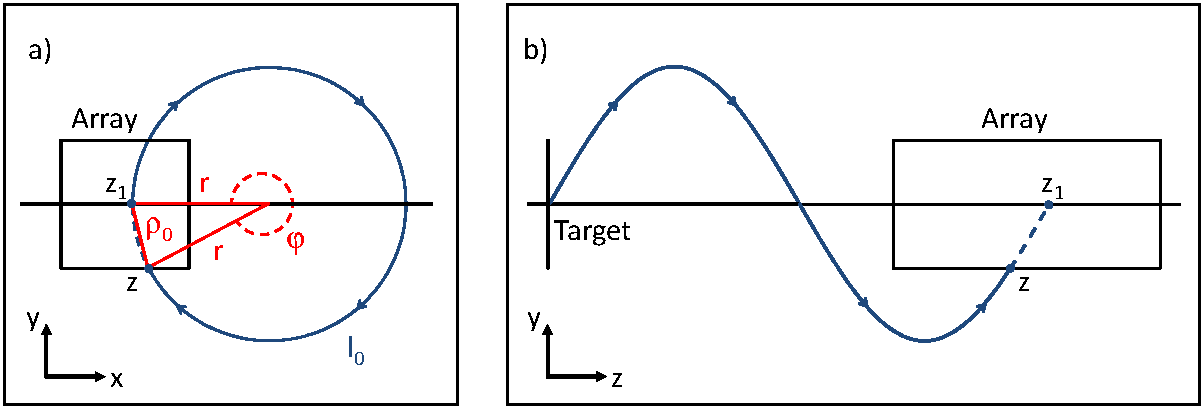
\includegraphics[width=\columnwidth]{array}
\caption[Illustration of a typical particle orbit intersecting a finite array]{Illustration of a typical particle orbit intersecting a finite array. a) The end-view of the array shows the transverse orbit length $l_0$ is truncated by the radius of the array $\rho_0$. b) The side-view of the array shows the relationship between $z$ the detection distance and $z_1$ the axis intercept.}%
\label{orbit_fig}%
\end{figure}
  The axis intercept $z_1$ is slightly greater in magnitude than the position where the particle is detected $z$ due to the finite transverse extent of any given detector array.  Similarly, the time of of flight $t$ is reduced from $T_\mathrm{cyc}$.  
\subsubsection{Formulation}
The effect of a finite detector array may be formulated in terms of its effect on the path length of a particle orbit.  The transverse path length of a particle orbit may be written as $l_0=\varphi r$ where $\varphi$ is the angle of rotation about the orbit's center.  For a detector of ``radius'' $\rho_0$, the path length of a single orbit $l_0$ is given by 
\begin{equation}
\begin{split}
{l_0}&=r(2\pi-\varphi_0)\\
&=r\left[2\pi-2\arcsin\left(\dfrac{\rho_0}{2r}\right)\right]\\
&\approx 2\pi r-\rho_0
\end{split}	
\label{trans_path}
\end{equation}
where $\varphi_0$ is the angle of the cyclotron orbit excluded by the detector array.  For a detector array with a non-circular (polygonal) cross section, the radius $\rho_0$ is a function of the azimuthal coordinate $\phi$.  In such case, a fixed $z$-position corresponds to a finite range of radii.  This leads to a variation in energy for a given transition at a fixed $z$, which is an example of kinematic broadening.
%For a detector array with a polygonal cross section $\rho_0$ is a function of $\phi$, the azimuthal coordinate.
  Thus, the detected position is given by 
\begin{equation}
\begin{split}
z&=v_\parallel t\\
&=v_\parallel \left(\frac{l_0}{v_{\perp}}\right)\\
%&=v_\| \left(\frac{r(2\pi-\phi)}{v_{\perp}}\right)\\
%z_\parallel
&=(v_{0}\cos(\theta_\mathrm{cm})+V_\mathrm{cm})\frac{r\left[2\pi-2\arcsin\left(\dfrac{\rho_0}{2r}\right)\right]}{v_0\sin(\theta_\mathrm{cm})}.
\end{split}	
\label{z_defined}
\end{equation}
\par As shown in Eq.~\ref{trans_path}, the transverse path length of the cyclotron orbit is reduced from 2$\pi r$ by approximately $\rho_0$, the radius of the detector array.  This approximation is valid when the quantity $\rho_0/2r$ is sufficiently small ($\ll1$).  Due to the acceptance limit imposed by a realistic detector array (see \S\,\ref{accept}), this condition is always true for detected particles.  Given this approximation, the relationship between the detected position of the ions $z$ and  the axis intercept $z_1$ is given by
\begin{equation}
\begin{split}
%&\approx(v_{0}\cos(\theta_\mathrm{cm})+V_\mathrm{cm})\frac{r\left[2\pi-2\left(\dfrac{\rho_0}{2r}\right)\right]}{v_0\sin(\theta_\mathrm{cm})}\\
z&\approx(v_{0}\cos(\theta_\mathrm{cm})+V_\mathrm{cm})\left(\frac{2\pi r-\rho_0}{v_0\sin(\theta_\mathrm{cm})}\right)\\
	 &=(v_{0}\cos(\theta_\mathrm{cm})+V_\mathrm{cm})\left(T_\mathrm{cyc}-\frac{\rho_0}{v_{0}\sin(\theta_\mathrm{cm})}\right)\\
&=v_\mathrm{lab}\cos(\theta_\mathrm{lab})\left(T_\mathrm{cyc}-\frac{\rho_0}{v_\mathrm{lab}\sin(\theta_\mathrm{lab})}\right)\\
%z_\parallel	 
&= z_1-\frac{\rho_0}{\tan(\theta_\mathrm{lab})}.
\end{split}	
\label{z_offset}
\end{equation}
Therefore, the deviation from the zero-radius detector limit is exaggerated for shallow emission angles with respect to the magnetic field axis, corresponding to smaller helical orbit radii.  The time of flight $t$ is reduced from the cyclotron period $T_\mathrm{cyc}$ in a similar fashion
\begin{equation}
\begin{split}
t&=T_\mathrm{cyc}-\frac{2r}{v_\perp}\arcsin\left(\frac{\rho_0/2}{r}\right) \\
&\approx T_\mathrm{cyc}-\dfrac{\rho_0}{v_0 \sin(\theta_\mathrm{cm})}
\end{split}
\label{time_of_flight}
\end{equation}

In the rearward hemisphere ($\theta_\mathrm{lab}>90^\circ$), the effect of a finite detector array manifests itself in the appearance of ``knees'' %or a ``fish-hook'' shape
 in the kinematic loci.  Fig.~\ref{analytic}(a) shows an analytic calculation of proton energies and center-of-mass angles vs. position for the $d$($^{28}$Si,$p$)$^{29}$Si reaction. The calculation assumes a cylindrical detector array of radius $\rho_0=$11.4\,mm and an ideal solenoid with a uniform field of 2.00\,T.  The effect of a non-zero radius detector array is illustrated by comparing the dotted lines in Fig.~\ref{analytic} with the solid lines corresponding to the ground-\-state transition.
 
In the forward hemisphere ($\theta_\mathrm{lab}<90^\circ$), the effect of a finite detector array is the same, insofar as the detected position $z$ is reduced in magnitude from the axis intercept $z_n$ as given in Eq.~\ref{z_offset}.  However, the velocity $v_\parallel$ and the slope $\partial E_\mathrm{lab}/\partial z$ have opposite sign, leading to a single-valued function of $E_\mathrm{lab}$ vs. $z$ at low energy.  In analogy to the knees mentioned above, this feature may be referred to as a ``heel'' shape.  Fig.~\ref{analytic}(c) shows an analytic calculation of helion energies and center-of-mass angles vs. position for the $d$($^{124}$Sn,$^3$He)$^{123}$In reaction. The calculation assumes a uniform field of 2.73\,T.

\begin{figure*}
\centering
%\includegraphics[width=\linewidth,keepaspectratio,height=0.5\textheight]{../NIM_Paper/Figures/Old_Figures/excel_plots_ab}
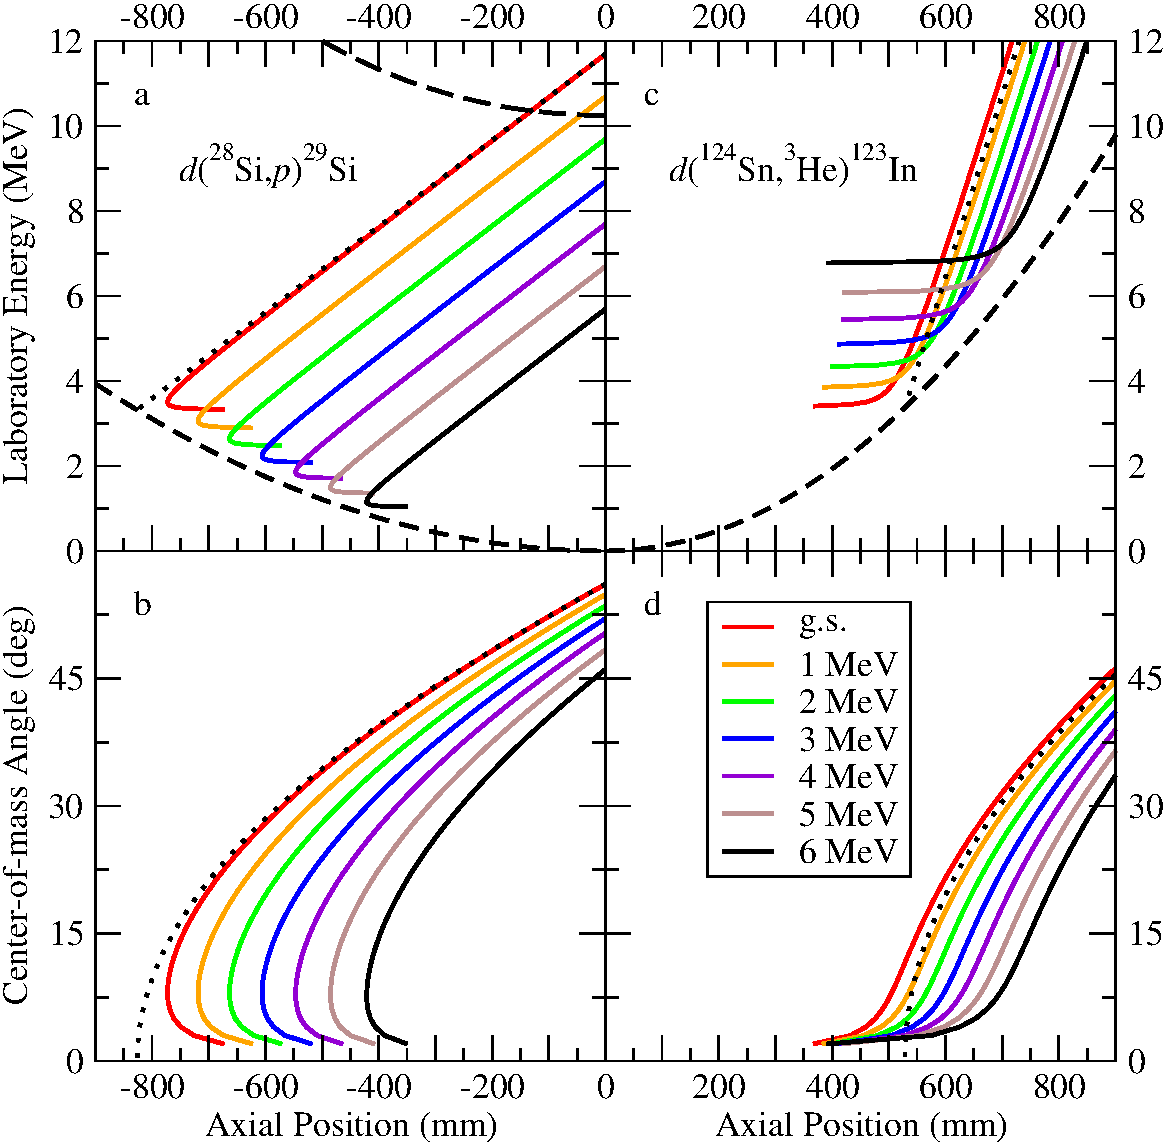
\includegraphics[angle=0,width=\textwidth,height=0.75\textheight,keepaspectratio]{4-kin_tall}
\caption[Calculated ejectile energies for the $d$($^{28}$Si,$p$)$^{29}$Si and $d$($^{124}$Sn,$^3$He)$^{123}$In reactions]{Calculated ejectile energies for the $d$($^{28}$Si,$p$)$^{29}$Si and $d$($^{124}$Sn,$^3$He)$^{123}$In reactions. Panels (a) and (b) correspond to $d$($^{28}$Si,$p$)$^{29}$Si,
 and panels (c) and (d) correspond to $d$($^{124}$Sn,$^3$He)$^{123}$In.
Panels (a) and (c) show the ejectile energy $E_\mathrm{lab}$ vs. detected axial position $z$ (relative to the target) for protons ejected in the rearward hemisphere and helions ejected in the forward hemisphere, respectively.  In panels (b) and (d), the emission angle of the ejectile in the center-of-mass $\theta_\textrm{cm}$ is plotted against the detected position $z$.  Excitation energies were selected such that $\Delta E_\mathrm{cm}=1$\,MeV.  The dotted line in each plot corresponds to the ground-\-state transition as measured by a detector array of zero radius, illustrating the difference between the axis intercept $z_1$ and the detected position $z$.  The dashed line running through panels (a) and (c) represents $\theta_\textrm{lab}=0^\circ$.  The upper dashed line in panel (a) corresponds to the limit imposed by the solenoid bore.  This limit occurs above the axis range in (c).  Both reaction calculations assume an ideal magnetic field of 2.00\,T.}
\label{analytic}
\end{figure*}

%In the forward hemisphere, the shape is 
\subsubsection{Compensation}
As discussed, the relationship given in Eq.~\ref{ecm} is an idealization which assumes a detector array of zero radius, meaning the detected position $z$ is equal to the axis intercept $z_1$.  The deviation from the zero-radius limit is effectively negligible for sufficiently large ejection angles.  The value of this ``threshold'' varies depending on the reaction, but can be seen to be about $\theta_\mathrm{lab}>10^\circ$ in Fig.~\ref{analytic}.  However, below this threshold, in the region of the knees, the offset is significant. In order to correct for this disparity, the time of flight must also be taken into account.  Using the relation $v_\parallel=z_1/T_\mathrm{cyc}=z/t$, Eq.~\ref{ecm} may be rewritten as 
\begin{equation}
E_\mathrm{cm}=E_\mathrm{lab}+\frac{1}{2} mV_\mathrm{cm}^2-\frac{m V_\mathrm{cm}}{t}z.
\label{ecm_new}
\end{equation}
Whereas Eq.~\ref{eq:no_comp} gives the $Q$-value resolution based only on the energy resolution, this reformulation of $E_\mathrm{cm}$ combines all three measured quantities.   

\begin{equation}
\begin{split}
\left(\delta E_\mathrm{cm}\right)^2&=\left(\frac{\partial E_\mathrm{cm}}{\partial E_\mathrm{lab}}\right)^2\left(\delta E_\mathrm{lab}\right)^2+\left(\frac{\partial E_\mathrm{cm}}{\partial z}\right)^2\left(\delta z\right)^2+\left(\frac{\partial E_\mathrm{cm}}{\partial t}\right)^2\left(\delta t\right)^2+2\left(\frac{\partial E_\mathrm{cm}}{\partial z}\right) \delta z \left(\frac{\partial E_\mathrm{cm}}{\partial t}\right)\delta t\\
\left(\delta E_\mathrm{cm}\right)^2&=\left(\delta E_\mathrm{lab}\right)^2+\left(\frac{-m V_\mathrm{cm}}{t}\right)^2\left(\delta z\right)^2+\left(\frac{m V_\mathrm{cm}}{t^2}z\right)^2\left(\delta t\right)^2+2\left(\frac{-m V_\mathrm{cm}}{t}\right) \delta z \left(\frac{m V_\mathrm{cm}}{t^2}z\right)\delta t
\end{split}
\label{eq:delta_z3}
\end{equation}

The excitation energy can be determined in the region of the knees with a sufficiently fine time resolution. Table~\ref{time_res} shows the contribution of the time resolution to the overall $Q$-value resolution.  However, with the prototype array discussed in \S\,\ref{charact} having a time resolution of $\delta t=3.87$\,ns, this correction has a prohibitively deleterious effect on the final $Q$-value resolution. 

\begin{table*}%
  \centering
  \begin{tabular}{lcc|cccrr}		
    \hline
    \multicolumn{1}{c}{\multirow{2}{*}{Reaction}}  &
    \multicolumn{1}{c}{$E_1/A_1$}  &
    \multicolumn{1}{c}{$\mathscr{B}$}  &
    \multicolumn{1}{c}{$\delta t$} & 
    \multicolumn{3}{c}{Origin of contribution}  &
    \multicolumn{1}{c}{$\delta E_\textrm{cm}$}  \\  \cline{5-7}
    &\multicolumn{1}{c}{(\AMeV)}&
    \multicolumn{1}{c}{(T)}&
    \multicolumn{1}{c}{(ns)}&
    \multicolumn{1}{c}{$\delta z$}  &  
    \multicolumn{1}{c}{$\delta E_\textrm{lab}$} & 
    \multicolumn{1}{c}{$\delta t$} & 
    \multicolumn{1}{c}{(keV)}\\
    \hline \hline 
    %\multirow{5}{*}{$d$($^{28}\textrm{Si}$,$p$)$^{29}\textrm{Si}$} 	 &3.87 & 50 & 5 & 480 & 485\\
    $d$($^{28}\textrm{Si}$,$p$)$^{29}\textrm{Si}$ &6.02&2.00
      &5.00 & 11 & 40 & 1,280 & 1,280\\
    &&&2.00 & 11 & 40 & 511 & 512\\
    &&&1.00 & 11 & 40 & 256 & 256\\
    &&&0.50 & 11 & 40 & 128 & 131\\
    &&&0.25 & 11 & 40 & 64 & 70\\
    \hline
  \end{tabular}
  \caption[Calculated contribution of $\delta t$ to the uncertainty in $E_\mathrm{cm}$]{Calculated contribution of $\delta t$ to the uncertainty in $E_\mathrm{cm}$.  Contributions are given in keV~FWHM and are tabulated 
    for several values of $\delta t$, holding $\delta E_\mathrm{lab}$ and 
    $\delta \theta_\mathrm{lab}$ fixed.  The values are calculated at $\theta_\mathrm{cm}=10^\circ$.}
  \label{time_res}
  \end{table*}

\subsection{Corrections for Relativity}
So far in this chapter, the effects of relativity have been ignored.  However, with heavy-ion reactions such as $^{132}$Sn($d$,$p$) planned to be measured with HELIOS at beam energies in the GeV-range, it is important to ensure that this premise is valid.  Stating the problem in terms of velocities and inertial frames, $v_\mathrm{lab}$ is the velocity of the projectile in the (stationary) laboratory frame; the center-of mass frame is moving with a velocity of $V_\mathrm{cm}$ relative to the laboratory frame in the $+z$ direction; and $v_0$ is the velocity of the ejectile in the center-of-mass frame.
\subsubsection{Transformation Factors}
Here, we have a choice of how best to keep the notation both brief and consistent.  The velocities $v_\mathrm{lab}$,$v_0$, and $V_\mathrm{cm}$ have been clearly defined; % and used consistently.  T
 therefore, the speed parameters may be written as $\beta$,$\beta_0$,$B_\mathrm{cm}$ and the Lorentz factors as $\gamma$,$\gamma_0$,$\Gamma_\mathrm{cm}$. 	
The velocity of the center-of-mass is defined in terms of the speed parameter $B_\mathrm{cm}=V_\mathrm{cm}/c$ where $c$ is the speed of light and $B_\mathrm{cm}$ is given by 
\begin{equation}
\begin{split}
B_\mathrm{cm}%&=\frac{P_1}{W_t}\\
%&=\frac{p_1c}{W_t}\\
&=\frac{p_1c}{\gamma_1 m_1c^2+m_2c^2}\\
&=\frac{\sqrt{E_1^2+2m_1c^2E_1}}{E_1+(m_1+m_2)c^2}.
\end{split}
\label{big_beta}
\end{equation}
Here the subscripts on $m_1$ and $m_2$ refer to the masses of the incident beam particle and the target particle, respectively.  The momentum $p_1$ and total energy $\gamma_1 m_1c^2$ of the beam particle are rewritten in terms of the total beam energy $E_1$ (\textit{cf}.~\citet[Eq.~7.98]{Goldstein_2002}).  The Lorentz factor for the center-of-mass frame is then written as $\Gamma_\mathrm{cm}=1/\sqrt{1-B_\mathrm{cm}^2}$.

\subsubsection{Energy}
With the total energy in the laboratory frame given by $W_t=E_1+(m_1+m_2)c^2$, the total energy in the center-of-mass frame is $W_t^\prime=W_t/\Gamma_\mathrm{cm}$.  Here, prime notation refers to quantities in the center-of-mass system.  With $W_t^\prime$ defined, the total energy of the ejectile in the center-of-mass is given by 
\begin{equation}
\begin{split}
W^\prime&=\frac{(W_t^\prime)^2+(m-M)c^2}{2W_t^\prime}
\end{split}
\label{eq:E_rel}
\end{equation}
where $m$ and $M$ are the mass of the ejectile and heavy recoil, respectively.  The excitation energy enters Eq.~\ref{eq:E_rel} implicitly via the heavy ion mass, given $M=M_0+E_x$.  Similarly, the reaction $Q$-value is represented in the particle masses (\textit{cf}. Eq.~\ref{eq:q_value}). Finally, the kinetic energy of the ejectile is given as a function of scattering angle as 
\begin{equation}
\begin{split}
E&=W-mc^2\\
&=W^\prime \Gamma_\mathrm{cm}(1+ B_\mathrm{cm} \beta_0 \cos(\theta_\mathrm{cm}))-mc^2
\end{split}
\label{eq:E_rel2}
\end{equation}

\subsubsection{Velocities}
The trajectories within HELIOS are defined by the velocity projections.  Using the standard ve\-loc\-i\-ty-ad\-di\-tion formula based on the Lorentz transformation, the axial velocity may be written as
\begin{equation}
\begin{split}
v_\parallel&=\frac{v_\parallel^\prime+V_\mathrm{cm}}{1+v_\parallel^\prime V_\mathrm{cm}/c^2}\\
&=\frac{v_0\cos(\theta_\mathrm{cm}) + V_\mathrm{cm}}{1+[v_0\cos(\theta_\mathrm{cm})]V_\mathrm{cm}/c^2}\\
&=\frac{v_0\cos(\theta_\mathrm{cm}) + V_\mathrm{cm}}{1+B_\mathrm{cm}\beta_{0}\cos(\theta_\mathrm{cm})}
%&=\frac{v_\parallel^\prime}{1+B_\mathrm{cm}\beta_{0}\cos(\theta_\mathrm{cm})}
\end{split}
\label{eq:rel_v_x}
\end{equation}
where $v_\parallel^\prime$ is the $z$-projection of the ejectile velocity in the center-of-mass frame.  Similarly, the radial velocity may be written as
\begin{equation}
\begin{split}
v_\perp&=\frac{v_\perp^\prime}{\Gamma_\mathrm{cm}(1+v_\parallel^\prime V_\mathrm{cm}/c^2)}\\
&=\frac{v_0 \sin(\theta_\mathrm{cm})}{\Gamma_\mathrm{cm}[1+B_\mathrm{cm}\beta_{0}\cos(\theta_\mathrm{cm})]}
\end{split}
\label{eq:rel_v_y}
\end{equation}
With these velocity transformations, the scattering angle in the laboratory $\theta_\mathrm{lab}$ is derived in the usual way
\begin{equation}
\begin{split}
\tan(\theta_\mathrm{lab})&=v_\perp/v_\parallel\\
&=\frac{v_0\sin(\theta_\mathrm{cm})}{\Gamma_\mathrm{cm}[v_0\cos(\theta_\mathrm{cm}) + V_\mathrm{cm}]}\\
&=\frac{1}{\Gamma_\mathrm{cm}}\frac{\sin(\theta_\mathrm{cm})}{\cos(\theta_\mathrm{cm})+K}
\end{split}
\label{eq:new_angle}
\end{equation}
Here $K$ retains its definition as $V_\mathrm{cm}/v_0$, but may be rewritten as $B_\mathrm{cm}/\beta_0$ (\textit{cf}.~\citet[Eq.~7.112]{Goldstein_2002}, \citet[Eq.~3.2]{Michalowicz_1967}).
\subsubsection{Cyclotron Orbit}
The cyclotron motion is defined by the velocity perpendicular to the magnetic field $v_\perp$.  As such, the relevant Lorentz factor is defined as $\gamma_\perp=1/\sqrt{1-(v_\perp/c)^2}$.  The equations of the cyclotron orbit may then be rewritten.
Eq.~\ref{cyc_rad} becomes
\begin{equation}
\begin{split}
r=v_{\perp}\frac{\gamma_\perp m}{\mathscr{B}q}\\
\end{split}
\label{rel_cyc_rad}
\end{equation}
and Eq.~\ref{Tcyc} becomes
\begin{equation}
T_\mathrm{cyc}=\frac{2\pi}{\mathscr{B}} \left(\frac{\gamma_\perp m}{q}\right)
\label{rel_Tcyc}
\end{equation}
%With these corrections the remainder of the equations relevant to calculating kinematics within HELIOS remain unchanged from \S\,\ref{}
\subsubsection{Example}
To use a representative example, consider the $^{124}$Sn($d$,$^3$He) reaction at 13\,\AMeV.  At the time of this writing, this reaction has the highest kinetic energy of any approved HELIOS experiment.  At the quoted energy, the $^{124}$Sn beam ion has a kinetic energy of $T=1.61$\,GeV and a rest mass of $m_0 c^2=115$\,GeV.  Even at this comparatively high energy, the collision is still in the classical energy regime of $T\ll m_0 c^2$, with $\gamma_0=1.01$.

With $K=1.42$, the energy solution is double-valued in the laboratory with a maximum ejection angle of $\theta_\mathrm{lab}=44.6^\circ$.  Taking relativistic kinematics into consideration, the maximum correction to the classically-calculated energy for a given $\theta_\mathrm{cm}$ scattering angle is 0.49\%.  For the high-energy solution, neglecting this correction corresponds to a calculation error of less than 500\,keV.  However, in the range of energies relevant to the prototype silicon detector array, which has a sensitivity of about 1--12\,MeV, this correction has an RMS value of 13\,keV\label{typo5}.  Therefore, for the purposes of calculating---and simulating---particle trajectories within HELIOS in order to determine an optimal experimental setup, the effects of relativity are negligible. 

\subsection{Technical Requirements}
It is useful here to briefly review the technical requirements to realize the HELIOS concept; these requirements are discussed in Ref.~\cite{Wuosmaa_2007} and summarized in Table~\ref{helios_req}.  The solenoid should have a radial parameter $\mathscr{B}r$ on the order of 1.25\,T$\cdot$m and a length parameter $\mathscr{B}L$ on the order of 3.5\,T$\cdot$m.  Standard ``3\,T'' Magnetic Resonance Imaging (MRI) medical scanners match these requirements.  For particle identification, a detector timing resolution of approximately 10\,ns is needed to separate particle groups with different values of $A/q$.  In order to straighten the knees of kinematic groups, timing resolution below 0.50\,ns is required; however, this feature is not necessarily required for successful operation of the spectrometer.  In order to take advantage of the $Q$-value resolution provided by the HELIOS measurement approach, certain limits need to be placed on the position and energy resolution of the detector array.  Position resolution on the order of 0.5--1.0\,mm~FWHM is required.  Energy resolution on the order of 25--50\,keV~FWHM is required.  The following chapters discuss how the actual performance characteristics of the HELIOS spectrometer compare to these requirements.

\begin{table}[b]
\centering
\begin{tabular}{ccccccccc}
\hline
\multicolumn{2}{c}{Solenoid}  &  &
\multicolumn{3}{c}{Detectors}  & & 
\multicolumn{2}{c}{Derived}\\ \cline{1-2} \cline{4-6} \cline{8-9}
\multicolumn{1}{c}{$\mathscr{B}R$}  &  
\multicolumn{1}{c}{$\mathscr{B}L$}  & &
\multicolumn{1}{c}{$\delta z$}  &  
\multicolumn{1}{c}{$\delta E_\textrm{lab}$} &
\multicolumn{1}{c}{$\delta t$} &&
\multicolumn{1}{c}{$\Delta \Omega$}  &  
\multicolumn{1}{c}{$\delta E_\mathrm{cm}$}  \\
(T$\cdot$m)&(T$\cdot$m)&&(mm)&(keV)&(ns)&&(sr)&(keV)\\
\hline \hline
1.25&3.5&&1.0&50&10.9&&0.99&100
\\
\hline 
\end{tabular}
\caption[Nominal performance specifications required to realize the HELIOS concept]{Nominal performance specifications required to realize the HELIOS concept.  These requirements are as outlined in this chapter and in Ref.~\cite{Wuosmaa_2007}.  The value of $\delta t$ is calculated based on the minimum separation of kinematic groups at $\mathscr{B}=3$\,T.  $\Delta \Omega$ is calculated for one target-to-detector setting for the simulated $^{132}$Sn($d$,$p$) reaction discussed in Ref.~\cite{Wuosmaa_2007}.}
\label{helios_req}
\end{table}